
%version 2: \usepackage{hyperref}


%%%%%%%%%%%%%%%%%%%%%%%%%%%%%%%%%%%%%%%%%%%%%%%%%%%%%%%%%%%%%%%%%%%%%%%%
%Para las ecuaciones siempre es Ec.(n).
%Para las figuras siempre es Fig.n, incluso en el caption de la figura. Tambien las Tablas
%Para las referencias es [n]
%%%%%%%%%%%%%%%%%%%%%%%%%%%%%%%%%%%%%%%%%%%%%%%%%%%%%%%%%%%%%%%%%%%%%%%%

\documentclass[
reprint,
%notitlepage,
%superscriptaddress,
%groupedaddress,
%unsortedaddress,
%runinaddress,
%frontmatterverbose, 
%preprint,
%showpacs,preprintnumbers,
%nofootinbib,
%nobibnotes,
%bibnotes,
%11 pt,
amsmath,
amssymb,
aps,
pra,
%prb,
%rmp,
%tightenlines %esto hizo el milagro de sacar los espacios en blancos estocásticos (?)
%prstab,
%prstper,
%floatfix,\textbf{}
]{revtex4-1} %Instalar primero para usarlo. Paquete malo.

%\documentclass[onecolumn, aps, amsmath,amssymb ]{article}
\usepackage{lipsum}  
\usepackage{graphicx}% Include figure files
\usepackage{subfig}
\usepackage{braket}
\usepackage{comment} %comment large chunks of text
\usepackage{dcolumn}% Align table columns on decimal point
\usepackage{bm}% bold math
%\usepackage{hyperref}% add hypertext capabilities
\usepackage[mathlines]{lineno}% Enable numbering of text and display math
%\linenumbers\relax % Commence numbering lines
\usepackage{mathtools} %% Para el supraíndice

\usepackage[nice]{nicefrac}

%%%%%%%El Señor Español%%%%%%%%%%%%%%%%%%%%%%%%%%%
\usepackage[utf8]{inputenc} %acento
\usepackage[
spanish, %El lenguaje.
es-tabla, %La tabla y no cuadro.
activeacute, %El acento.
es-nodecimaldot %Punto y no coma con separador de números
]{babel}
\usepackage{microtype} %para hacerlo más bonito :33 como vos (?) 
%%%%%%%%%%%%%%%%%%%%%%%%%%%%%%%%%%%%%%%%%%%%%%%%%%%
%%%%%%%%% Para que las imágenes se queden dónde las quiero (?
\usepackage{float}
%%%%%%%%%%

\usepackage{hyperref} % Para usar \url

%%%%%%%%Cambia a Fig de Figure%%%%%%%%%%
\makeatletter
\renewcommand{\fnum@figure}{Fig. \thefigure} 
\makeatother
%%%%%%%%%%%%%%%%%%%%%%%%%%%%%%%%%%%%%%%%
\raggedbottom

\usepackage{multirow}

\begin{document}
%%%%%%%%%%%%%%%%%%%%%%%%%%%%%%%%%%Título%%%%%%%%%%%%%%%%%%%%%%%%%%%%%%%%%%%%%%
%%%%%%%%%%%%%%%%%%%%%%%%%%%%%%%%%%%%%%%%%%%%%%%%%%%%%%%%%%%%%%%%%%%%%%%%%%%%%%

\title{Resultados del método East-West con All Triggers}
\author{Evelyn~G.~Coronel}

\affiliation{
Tesis de Maestría en Ciencias Físicas\\ Instituto Balseiro\\}

\date[]{\lowercase{\today}} %%lw para lw, [] sin date

%\begin{abstract}

%\end{abstract} 
\maketitle
%%%%%%%%%%%%%%%%%%%%%%%%%%%%%%%%%%%%%%%%%%%%%%%%%%%%%%%%%%%%%%%%%%%%%%%%%%%%%%%%%%%
% Podemos usar cualquiera de los dos comandos: \input o \include para incluir el texto

\section*{Como se hace el cálculo}

\begin{enumerate}
    \item Definimos el rango de tiempo a estudiar, para estos resultados se utilizaron los límites: 1 de Enero del 2014 hasta el 1 de Enero del 2020.
    \item Se recorre cada evento que cumpla con las siguientes características:
     \begin{itemize}
        \item Pertenezca el rango de energía a estudiar
        \item Sea un evento 6T5 con ángulo cenital menor a $60^o$
        \item Se haya registrado en el rango de tiempo seleccionado
    \end{itemize}
    En cada evento se calcula los siguientes valores:
    \begin{align}
        a' = \cos(X - \beta)\\
        b' = \sin(X - \beta)
    \end{align}
    el valor de $X$ depende la frecuencia a estudiar, la misma es igual a la ascensión recta del cenit $\alpha^0_i$ al momento del evento  si se estudia la frecuencia sidérea, en cambio para la frecuencia solar es igual al equivalente en grados de la hora local de Malargüe. El valor de $\beta$ es depende si el evento provino del Este donde $\beta=180^o$ o $\beta=0$ caso contrario.
    Se intentó hacer un barrido de frecuencias análogo al análisis de Rayleigh pero la variable utilizada para generalizar el análisis a frecuencias arbitrarias:
    \begin{equation}
        \tilde{\alpha} = 2\pi f_x t_i + \alpha_i - \alpha_i^0(t_i) \label{ra_mod}
      \end{equation}
    es tal que la variable es igual a la ascensión recta del evento a estudiar y no al cenit como es el caso del EW. 
    \item Una vez corridos todos los  eventos se calculan los parámetros:
    \begin{align*}
        a_{EW} &= \frac{2}{N} \sum^N_{i=1} a \qquad
        b_{EW} = \frac{2}{N} \sum^N_{i=1} b
    \end{align*}
    que es equivalente a haber calculado
    \begin{align*}
        a_{EW} &= \frac{2}{N} \sum^N_{i=1} \cos(\alpha^0_i - \beta_i)\\
        b_{EW} &= \frac{2}{N} \sum^N_{i=1} \sin(\alpha^0_i - \beta_i)
    \end{align*}
    donde N indica la cantidad eventos considerados. La cantidad de eventos por rango de energía se muestran en la tabla \ref{tab:}.

    Con esto puedo calcular la amplitud asociada al análisis $r_{EW}$ y la fase $\phi_{EW}$:
    \begin{align*}
        r_{EW} = \sqrt{a_{EW}^2 + b_{EW}^2}\\
        \phi_{EW} = \tan^{-1}(\nicefrac{b_{EW}}{a_{EW}})
    \end{align*}

    Estos valores se traducen a los valores de amplitud $r$ y fase $\phi$ del dípolo físico mediante las expresiones:
    \begin{align*}
        r = \frac{\pi}{2} \frac{\langle\cos\delta \rangle}{\langle\sin\theta \rangle} &r_{EW} \qquad
        \phi = \phi_{EW} + \frac{\pi}{2}\\
        d_\perp&= \frac{\pi}{2 \langle\sin\theta \rangle} r_{EW}
    \end{align*}
    Se suma $\frac{\pi}{2}$ por el  artificio de agregar $\pi$ en los coeficientes para obtener la diferencia entre tasas del este y oeste. Los valores $\langle\cos\delta \rangle$ y $\langle\sin\delta \rangle$ son los valores medios de estas variables en los años estudiados. 

    \item Se calcula la amplitud límite $r_{99}$ y la probabilidad de que las amplitudes calculadas sea ruido  $P(r_{EW})$ mediante:
    \begin{align*}
        P(\geq r_{EW}) = \exp{-\frac{N}{4}r^2_{EW}}\\
        r_{99} = \frac{\pi}{2} \frac{\langle\cos\delta \rangle}{\langle\sin\theta \rangle}\sqrt{\frac{4}{N}\ln(100)}
    \end{align*}

\end{enumerate}

% Por último, estos resultados se comparan con los valores obtenidos con el método EW en el trabajo \cite{Aab_2020} en frecuencia sidérea, aplicado al conjunto de eventos del disparo estándar registrados entre el 1 de Enero del 2004 y el 1 de Agosto del 2018. Para esto se ejecutó el programa implementado en el trabajo mencionado sobre los datos utilizados en el mismo, estos se obtuvieron de \emph{Publications Committee} de la colaboración Auger.


Por último, estos resultados se comparan con los valores obtenidos con el método EW en el trabajo \cite{Aab_2020} en frecuencia sidérea, aplicado al conjunto de eventos del disparo estándar registrados entre el 1 de Enero del 2004 y el 1 de Agosto del 2018. 
% Para esto se ejecutó el programa implementado en el trabajo mencionado sobre los datos utilizados en el mismo, estos se obtuvieron de \emph{Publications Committee} de la colaboración Auger.


\section*{Verificación del código}
Se verificó el código escrito en este trabajo de la siguiente manera:

\begin{enumerate}[noitemsep]
    \item El conjunto de eventos del disparo estándar registrados entre el 1 de Enero del 2004 y el 1 de Agosto del 2018 fue analizado en el trabajo \cite{Aab_2020}.
    \item Utilizando el código y los datos de los eventos del paper \cite{Aab_2020}, obtenidos de la página del \emph{Publications Committee} de la colaboración Auger, se replicaron los datos del paper. 
    \item Luego utilizando el código escrito para este trabajo, se realiza que análisis de EW con los datos del trabajo \cite{Aab_2020}. 
    \item Finalmente se verificó que los valores obtenidos en los item 2 y 3, con  ambos códigos, sean el mismo.
\end{enumerate}


\section*{Tabla cantidad de eventos para distintos rangos de energía}

Los eventos son clasificados en los distintos rangos con la energía reportada el archivo del Herald de todos los disparos  entre el 2014 y 2019 y para el disparo estándar entre el 2004 y 2018.
\begin{table}[H]
    \begin{small}
        \begin{center}
            \begin{tabular}{ll|c|c|c|}
                \cline{3-5}
                \multicolumn{2}{l|}{Rango {[}EeV{]}}                                                                        & 0.25 - 0.5    & 0.5 - 1       & 1 - 2         \\ \hline
                \multicolumn{1}{|l|}{\multirow{2}{*}{Eventos}}                                                  & Todos    & $3\,967\,368$ & $3\,638\,226$ & $1\,081\,846$ \\ \cline{2-5} 
                \multicolumn{1}{|l|}{}                                                                          & Estándar & $770\,323$    & $2\,388\,468$ & $1\,243\,098$ \\ \hline \hline
                \multicolumn{1}{|l|}{\multirow{2}{*}{\begin{tabular}[c]{@{}l@{}}Energía \\ Media\end{tabular}}} & Todos    & $0.38$       & $0.69$       & $1.32$       \\ \cline{2-5} 
                \multicolumn{1}{|l|}{}                                                                          & Estándar & $0.42$        & $0.71$        & $1.34$.       \\ \hline
                \end{tabular}
            \caption{Tabla de eventos por rango de energía }
            \label{tab:}
        \end{center}
    \end{small}
\end{table}
\subsection*{Resultados en el rango 0.25 EeV - 0.5 EeV}

En la Fig. \ref{fig:primer} se comparan las direcciones en las que apuntan la fase en frecuencia siderea obtenida en este trabajo con la obtenida en \cite{Aab_2020}. 
Las fases tiene un margen donde se solapan en la incertidumbre pero no son comparables, la línea punteada marca la dirección del centro galáctico.

\begin{table}[H]
    \begin{small}
        \begin{center}
            \begin{tabular}[c]{l|c||c|c}
                Frecuencia:         & 365.25	  & 366.25	   & 366.25 \cite{Aab_2020}   \\
                Amplitud [\%]:      & 0.173	      & 0.123	   & 0.50      \\
                $d_\perp$[\%]:      & -	          & 0.156	   & $0.6^{+0.6}_{-0.3}$       \\
                Probabilidad [\%] : & 66\%        & 81\%	   & 45\%       \\
                Fase[$^o$]:               & 145$\pm$60         & 279$\pm$90 & 226$\pm$50   	\\
                $r_{99}$ [\%]:      & 0.58	      & 0.58       & 1.2       \\
                $d_{\perp,99}$[\%]: & -           & 0.73       & 1.5      \\
            \end{tabular}
        \end{center}
    \end{small}
    \caption{Características para las frecuencias solar y sidérea con el método East-West en el primer armónico en rango de energía 0.25 EeV - 0.5 EeV}
    \label{tab:solar}
\end{table}


\subsection*{Resultados en el rango 0.5 EeV - 1 EeV}
En este rango de energía se observa una diferencia entre las probabilidades de este trabajo y \cite{Aab_2020}  ne la frecuencia sidérea. Este valor dice cuando probable es que las amplitudes sean debido al ruido. Este trabajo obtiene que la amplitud en sidérea es significativa por un  $6\%$.  

En la Fig. \ref{fig:segundo} se comparan las direcciones en las que apuntan la fase en frecuencia sidérea obtenida en este trabajo con la obtenida en \cite{Aab_2020}. En esta figura se observa que las fases son comparables entre sí y apuntan a una dirección cercana al centro galáctico (línea punteada).


\begin{figure}[H]
    \begin{small}
        \begin{center}
            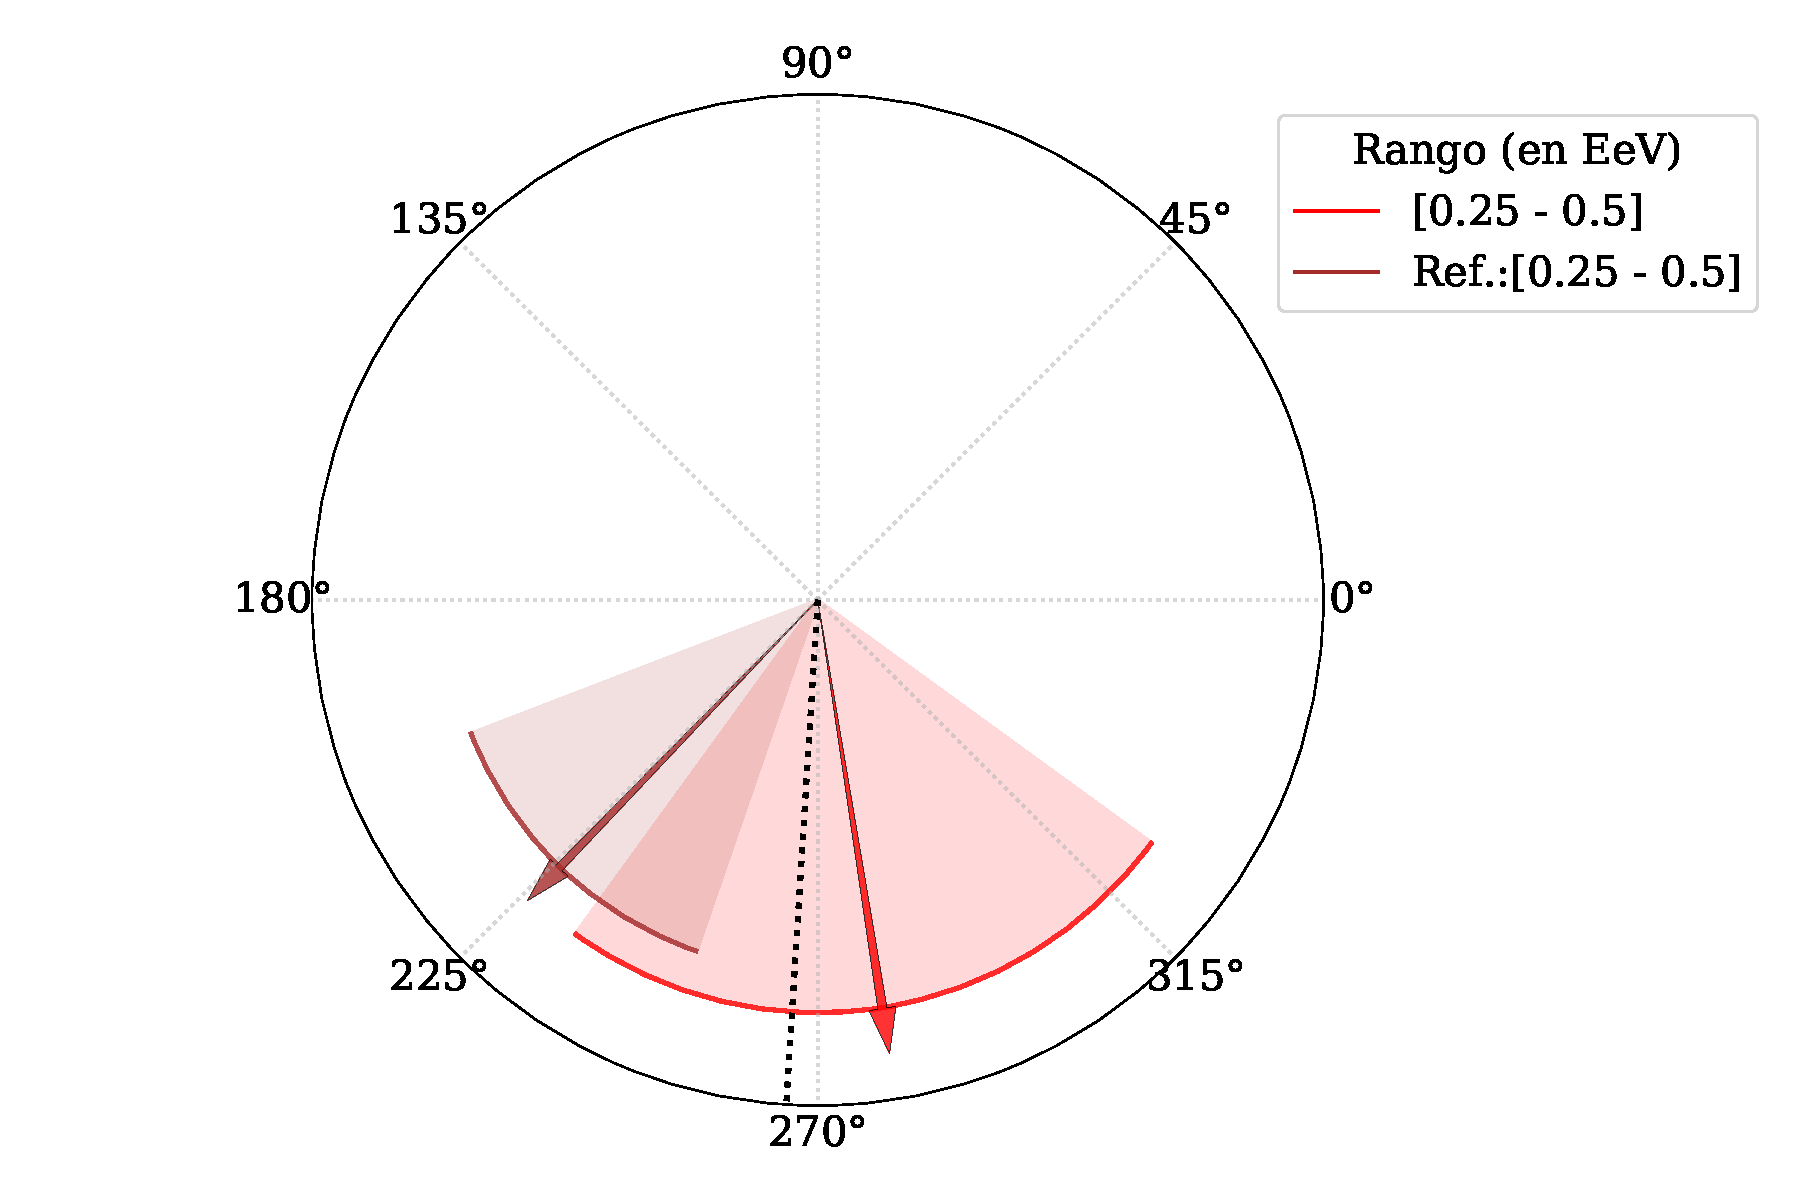
\includegraphics[width=0.5\textwidth]{phase_primer_bin.pdf}
        \end{center}
        \caption{Valores de las fases obtenidos en este trabajo y en la referencia con sus respectivas incertidumbres para la frecuencia sidérea en el  rango 0.25 EeV - 0.5 EeV .}
        \label{fig:primer}
    \end{small}
\end{figure}

\begin{figure}[H]
    \begin{small}
        \begin{center}
            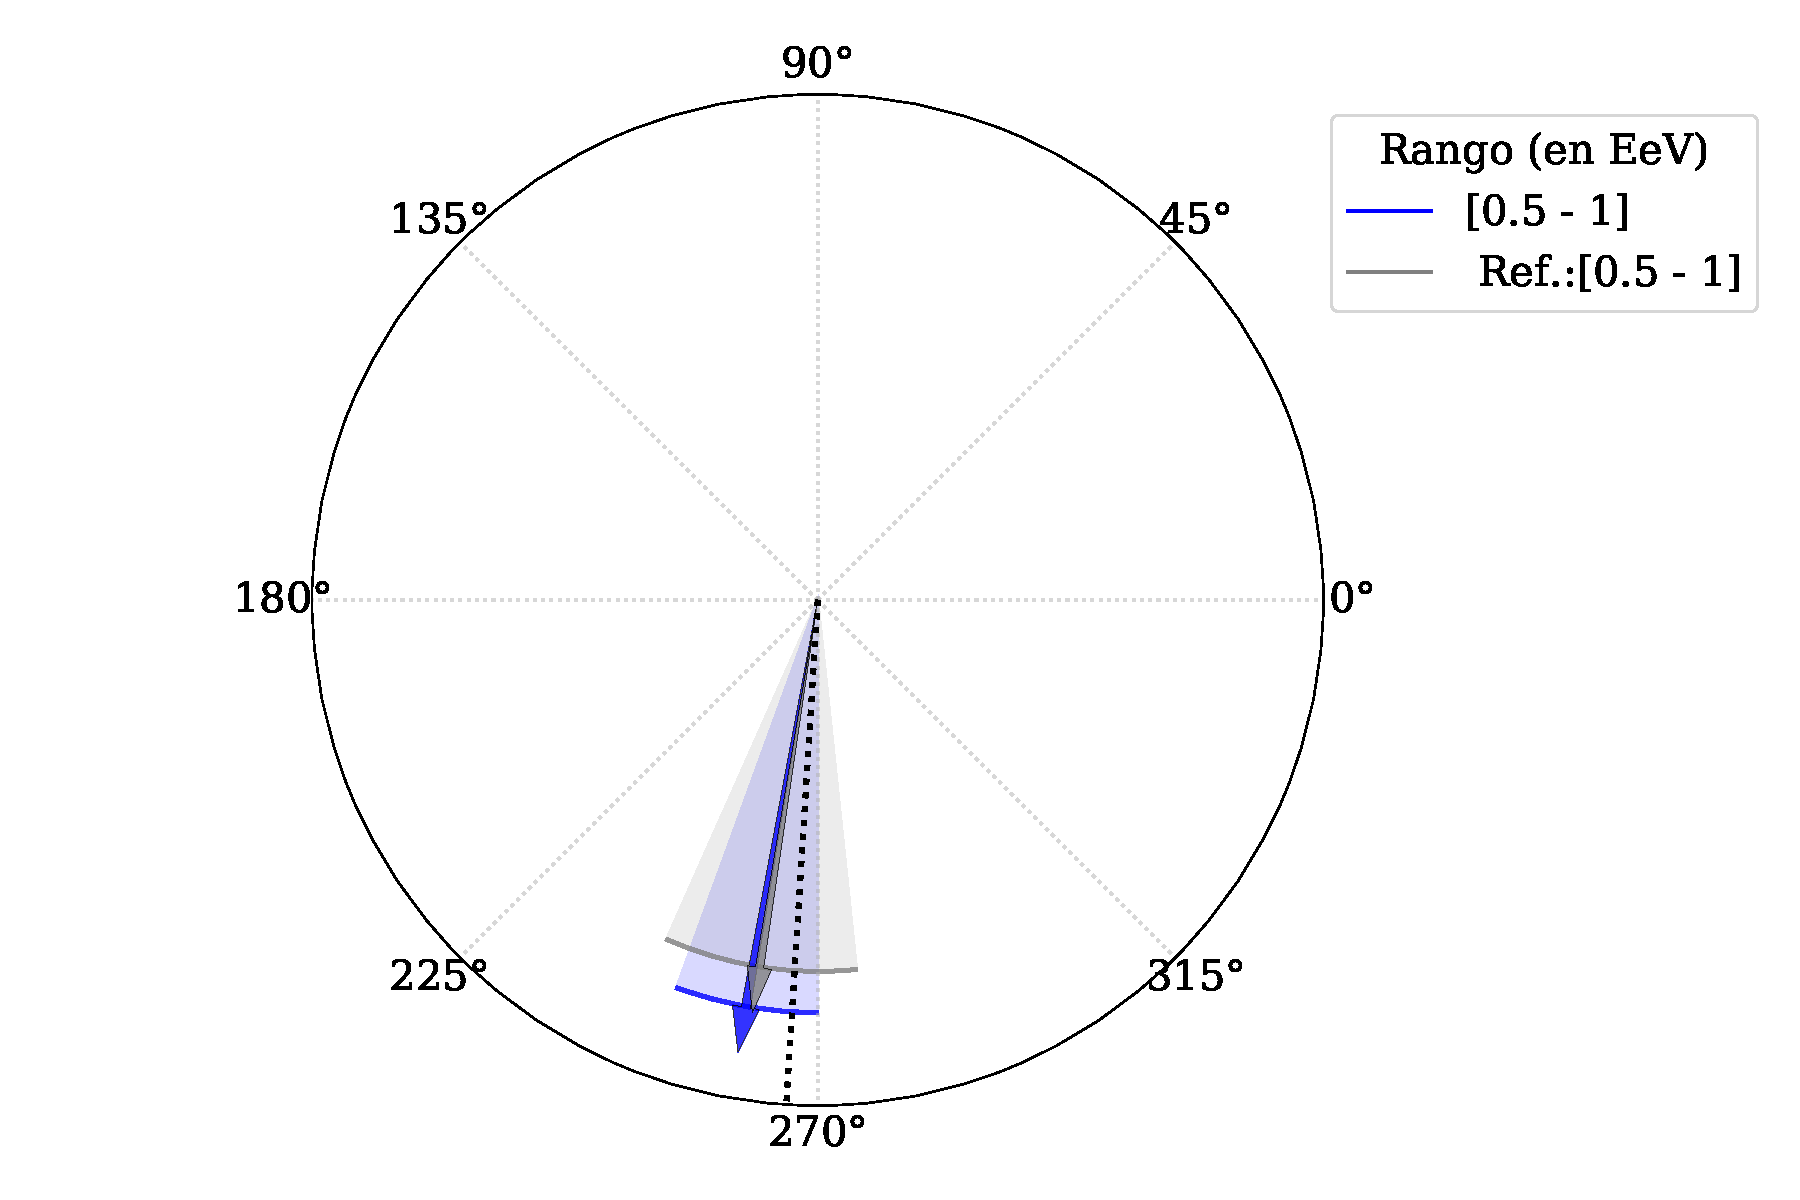
\includegraphics[width=0.5\textwidth]{phase_segundo_bin.pdf}
        \end{center}
        \caption{Valores de las fases obtenidos en este trabajo y en la referencia con sus respectivas incertidumbres para la frecuencia sidérea en el  rango 0.5 EeV - 1.0 EeV .}
        \label{fig:segundo}
    \end{small}
\end{figure}

\begin{table}[H]
        \begin{small}
            \begin{center}
                \begin{tabular}[c]{l|c||c|c}
                    Frecuencia:     & 365.25	    & 366.25		& 366.25\cite{Aab_2020}\\
                    Amplitud [\%]:  & 0.40          & 0.40	        & 0.40\\
                    $d_\perp$[\%]:  & -             & 0.60          & $0.50^{+0.3}_{-0.2}$\\
                    Probabilidad:   & 7\%           & 6\%	        & 20\%\\
                    Fase[$^o$]:     & 128$\pm$20	& 260$\pm$20	& 260$\pm$30\\
                    r99[\%]:        & 0.60	        & 0.60          & 0.6\\
                    $d_{\perp,99}[\%]$  & -         & 0.71          & 0.81\\
                \end{tabular}
            \end{center}
        \end{small}
        \caption{Características para las frecuencias solar y sidérea con el método East-West en el primer armónico en rango de energía 0.5 EeV - 1 EeV}
        \label{tab:solar}
    \end{table}

    


\subsection*{Resultados en el rango 1 EeV - 2 EeV}

 
En las Tablas \ref{tab:solar_3} y \ref{tab:siderea_3} se comparan los resultados de este trabajo y los obtenidos en \cite{Aab_2020} para la frecuencia solar y sidérea respectivamente. En el Fig.\ref{fig:tercer} se observan en un gráfico polar las fases de la referencia y este trabajo para la frecuencia sidérea. Los resultados son comparables entre sí.
    
    \begin{table}[H]
        \begin{small}
            \begin{center}
                \begin{tabular}[c]{l|c|c}
                                    & Rayleigh      & EW            \\\hline
                    Frecuencia:     & 365.25	    & 365.25        \\
                    Amplitud:       & 0.00385       & 0.00282       \\
                    Probabilidad:   & 0.02          & 0.64          \\
                    Fase:           & 288$\pm$20    & 200$\pm$60    \\
                    r99:            & 0.0041263     & 0.00916       \\
                \end{tabular}
            \end{center}
        \end{small}
        \caption{Características para la frecuencia solar con los métodos de Rayleigh  e East-West en el primer armónico.}
        \label{tab:solar_3}
    \end{table}

    \begin{table}[H]
        \begin{small}
            \begin{center}
                \begin{tabular}[c]{l|c||c|c}
                                    & Rayleigh     & EW         & EW\cite{Aab_2020}      \\\hline
                    Frecuencia:     & 366.25	   & 366.25     & 366.25      \\
                    Amplitud:       & 0.0040	   & 0.00495    & 0.00143      \\
                    $d_\perp$:      & 0.0051       & 0.00631    & 0.00182      \\ 
                    Probabilidad:   & 0.012	       & 0.26       & 0.87          \\
                    Fase:           & 330$\pm$20   & 320$\pm$30 & 290$\pm$100      \\
                    r99:            & 0.0041	   & 0.00916    & 0.00837      \\
                    $d_{\perp,99}$  & 0.0053       & 0.0117     & 0.0107       \\
                \end{tabular}
            \end{center}
        \end{small}
        \caption{Características para la frecuencia sidérea con los métodos de Rayleigh  e East-West en el primer armónico.}
        \label{tab:siderea_3}
    \end{table}

    La referencia tiene $1\,243\,098$ eventos con una energía media de $1.34$.

   
    \begin{figure}[H]
        \begin{small}
            \begin{center}
                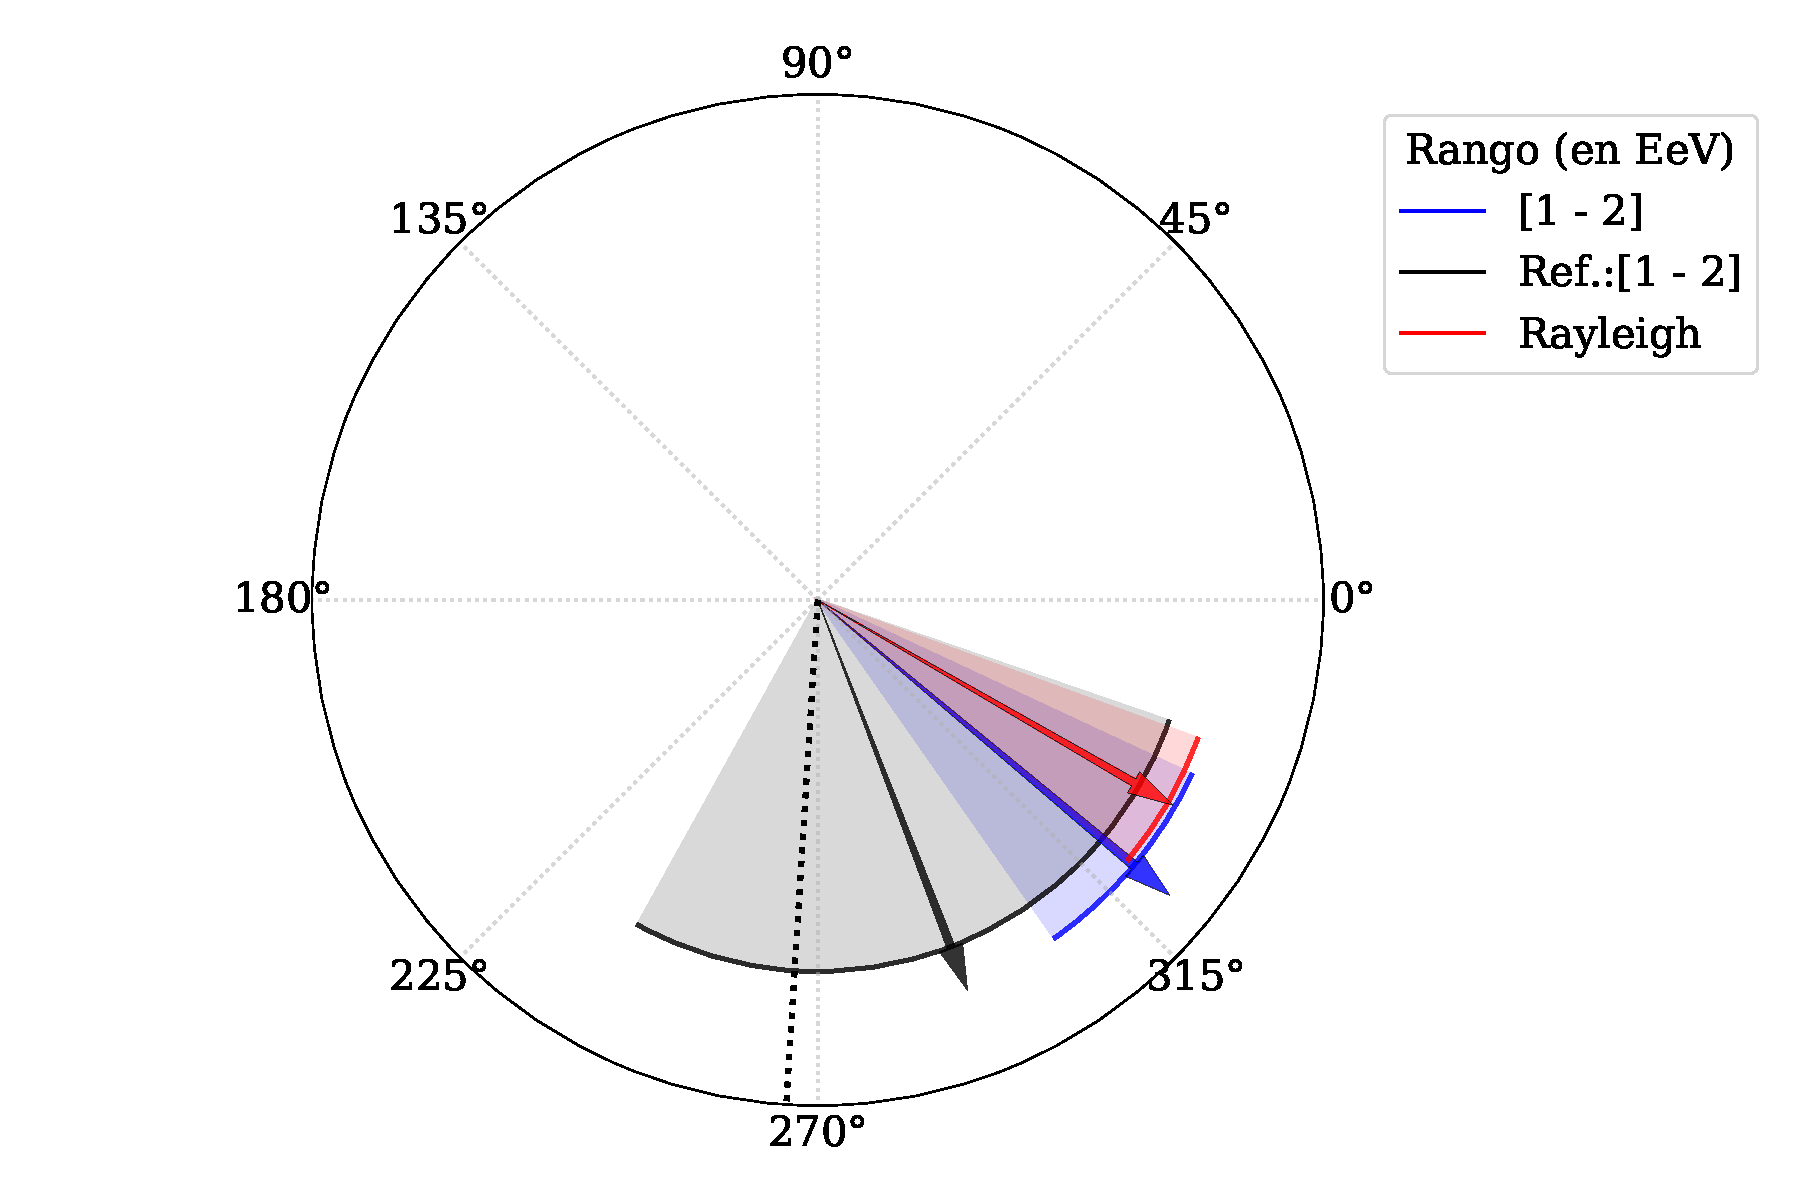
\includegraphics[width=0.5\textwidth]{phase_tercer_bin.pdf}
            \end{center}
        \caption{Valores de las fases obtenidos en este trabajo y en la referencia con sus respectivas incertidumbres para la frecuencia sidérea en el  rango 1.0 EeV - 2.0 EeV .}
        \label{fig:tercer}
        \end{small}
    \end{figure}


    \section*{Gráficos}

    Para poder comparar los resultados de $d_\perp$ entre sí, podríamos graficar los valores de la proyección y de la límite del $99\%$ como se muestra en la Fig.\ref{fig:no_normalizado}. El inconveniente es la cantidad de datos en cada rango de energía entre los conjuntos de datos, todos los disparos y disparo estándar, son distintos.

    \begin{figure}[H]
        \begin{small}
            \begin{center}
                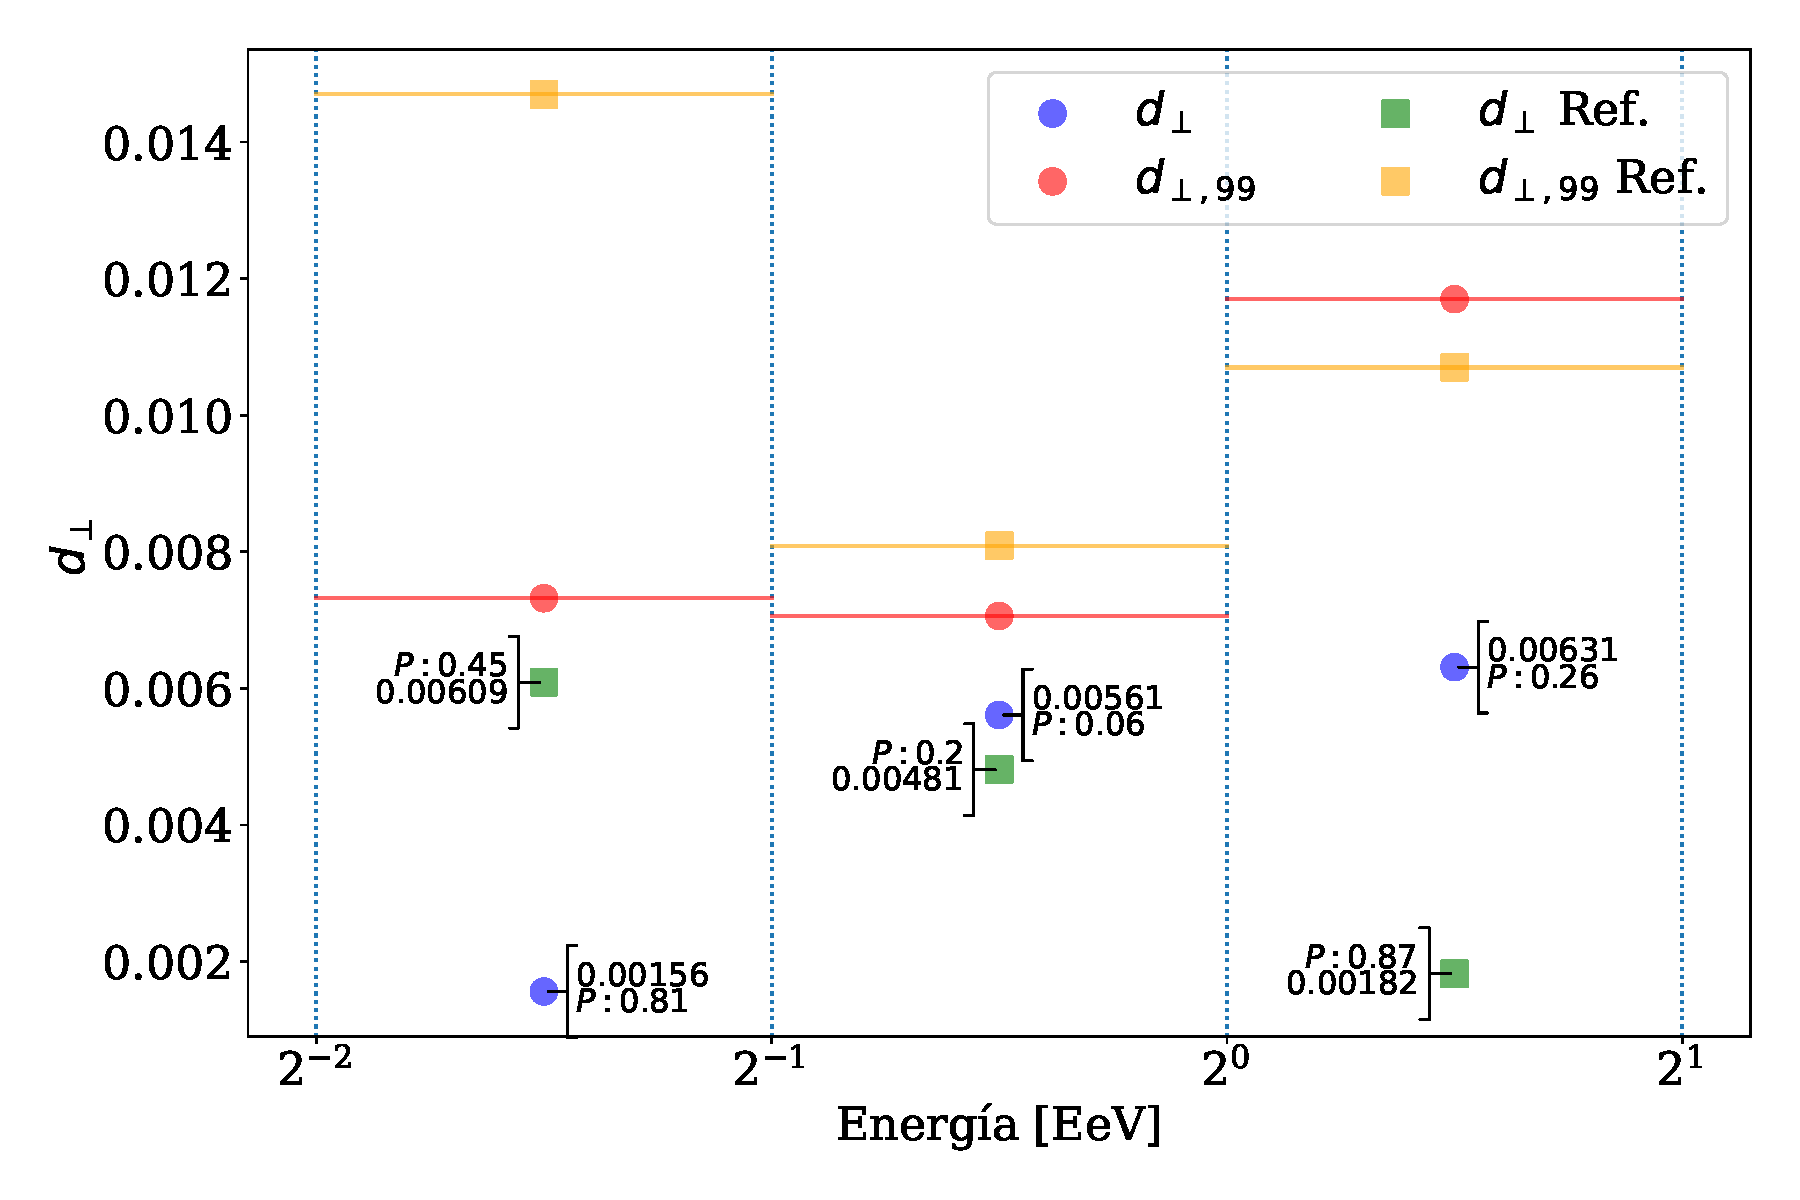
\includegraphics[width=0.5\textwidth]{d_perp_no_normalizado_v2.pdf}
            \end{center}
            \caption{Sin normalizar}
            \label{fig:no_normalizado}
        \end{small}
    \end{figure}
    
    Para compararlos mejor con respecto a $d_{\perp,99}$, usamos el valor de cada rango y de cada conjunto de datos, para normalizar la amplitud de $d_{\perp,99}$. Como se muestra en la Fig.\ref{fig:normalizado}, ahora $d_{\perp,99}=1$ y los otros valores se pueden comparar. 

    \begin{figure}[H]
        \begin{small}
            \begin{center}
                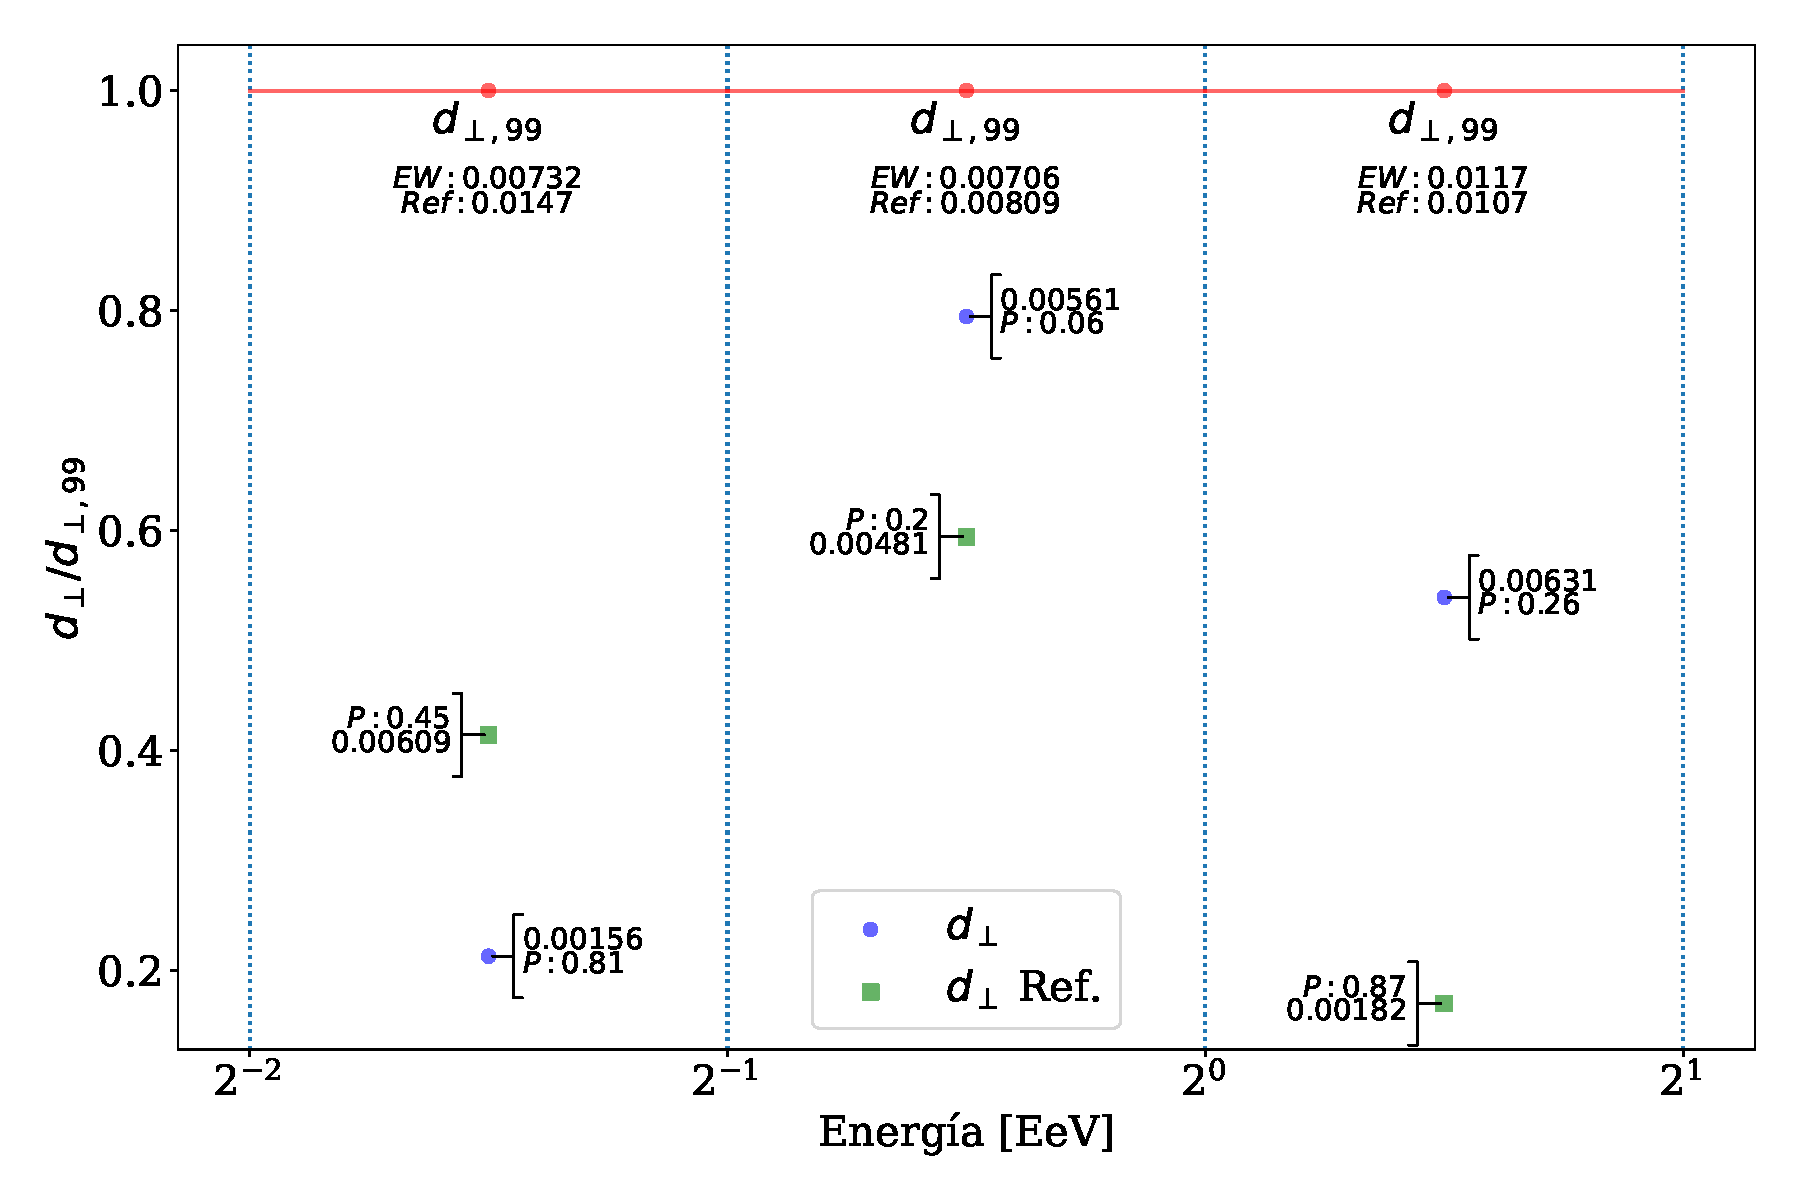
\includegraphics[width=0.5\textwidth]{d_perp_normalizado.pdf}
            \end{center}
            \caption{Valores normalizados con $d_{\perp,99}$}
            \label{fig:normalizado}
        \end{small}
    \end{figure}
    

Por lo que ahora podemos decir que en los rangos entre 0.5 EeV - 1.0 EeV y 1.0 EeV - 2.0 EeV, la amplitud obtenida en este trabajo está por encima que la referencia. 

Para comparar los resultados en el  rango 0.25 EeV - 0.5 EeV, tenemos que tener en cuenta que el disparo estándar tiene una sensibilidad menor que el todos los disparos. Esto se ve claramente en la Tabla \ref{tab:}, donde el primer tiene 7 veces menos eventos para analizar. Por lo tanto, la discrepancia entre la referencia y los trabajos puede deberse a la  diferencia de eventos a estudiar causada por la sensibilidad del disparo.


    \bibliographystyle{apsrev4-1}
    \bibliography{mibib.bib}
    
    \end{document}
